% !TEX root = ../../../main.tex

\section{Пропозициональные формулы}
Есть знаки логических $\wedge, \vee, \rightarrow, \neg$, действий и скобки.
\subsection{Формулы с одной бинарной связкой}
\begin{definition}
    Правильные алгебраические выражения (ПАВ) --- формулы с одной бинарной связкой. Они задаются рекурсивным правилом:
\begin{enumerate}
    \item $p$ --- переменная $\Rightarrow p$ --- ПАВ
    \item $\phi, \psi$ --- ПАВы $\Rightarrow (\phi * \psi)$ --- ПАВ
\end{enumerate}
По записи $((a*b)*(c*(d*e)))$ можно однозначно построить дерево.
\end{definition}

\begin{theorem}
    ПАВы и деревья разбора взаимно однозначно сопоставляются друг другу. Мы докажем, что для любого ПАВ $\eta$ не являющегося переменной, существует единственная пара $(\phi, \psi)$, такая, что $\eta \eqcirc  (\phi * \psi)$
\end{theorem}
\begin{proof}
\begin{lemma}[О балансе скобок]
    Баланс любого префикса ПАВ $\ge 0$. При этом баланс равен 0 только для $\varepsilon$ и всего ПАВ.
\end{lemma}
\begin{proof}
Доказательство по индукции по построению
    \begin{enumerate}
        \item[] \textbf{База:} $p$ --- переменная --- 2 префикса: $\varepsilon$, ПАВ, лемма верна 
        \item[] \textbf{Переход:} пусть для $\phi, \psi$ лемма верна. Докажем для $(\phi*\psi)$. Рассмотрим префиксы: $\varepsilon, ($, потом баланс будет $\ge 1$ по предположению индукции (и так как у нас есть одна открывающая скобка) никогда не будет равен 0, только в начале $\phi$ и в конце, следовательно, он обнулится только, когда для самой первой скобки найдется пара, то есть в самом конце.
    \end{enumerate}
\end{proof}
Теперь, пусть $A = (\phi*\psi) \eqcirc (\zeta'*\xi') = B$
Б.О.О. у $A$ звездочка, разделяющая $\phi, \psi$ стоит на месте $k$, а у  $B$ --- на месте $l$. Б.О.О $k < l$. Но тогда $a_2a_3a_4\dots a_k$ --- ПАВ. Но тогда $a_2a_3a_4\dots a_k = \phi \sqsubset \zeta$, но по лемме о балансе у каждого выражения баланс 0 достигается только в начале и в конце. Противоречие, значит $\phi \eqcirc \zeta$
\end{proof}
\subsection{Пропозициональные формулы}
\begin{enumerate}
    \item $p$ --- переменная $\Rightarrow p$ --- ПФ
    \item $\phi, \psi$ --- ПФы $\Rightarrow (\phi \wedge \psi), (\phi \vee \psi), (\phi \rightarrow \psi), $ --- ПФы
    \item $\phi$ --- ПФ $\Rightarrow \neg\phi$ --- ПФ
\end{enumerate}
\begin{lemma}[О балансе скобок]
    Баланс любого префикса ПФ $\ge 0$. При этом баланс равен 0 только для $\varepsilon$, всего ПФ и цепочки отрицаний ($\neg\neg\neg\dots\neg$).
\end{lemma}
\begin{proof}
Доказательство представляется читателю в качестве несложного упражнения
\end{proof}
\subsection{Булевы функции}
$f: \{0, 1\}^k \rightarrow \{0, 1\}$ --- булева функция от $k$ переменных. Тогда общее число функций $= 2^{2^k}$. Для $k = 1$ общее количесвто функций равно 4.
$$\begin{array}{c|cccc}
    p & \perp & p & \neg p & \top\\
    \hline
    0 & 0 & 0 & 1 & 1 \\
    1 & 0 & 1 & 0 & 1
\end{array}$$

Для $k = 2$ общее количесвто функций равно 16.
$$\begin{array}{cc|cccccccccccccccc}
    p & q & \perp & \top & p & q & \neg p & \neg q & \wedge & \vee & \oplus & \rightarrow & \leftarrow & \leftrightarrow & \not\rightarrow & \not\leftarrow & \downarrow & \uparrow\\
    \hline
    0 & 0 & 0 & 1 & 0 & 0 & 1 & 1 & 0 & 0 & 0 & 1 & 1 & 1 & 0 & 0 & 1 & 1\\
    0 & 1 & 0 & 1 & 0 & 1 & 1 & 0 & 0 & 1 & 1 & 1 & 0 & 0 & 0 & 1 & 0 & 1\\
    1 & 0 & 0 & 1 & 1 & 0 & 0 & 1 & 0 & 1 & 1 & 0 & 1 & 0 & 1 & 0 & 0 & 1\\
    1 & 1 & 0 & 1 & 1 & 1 & 0 & 0 & 1 & 1 & 0 & 1 & 1 & 1 & 0 & 0 & 0 & 0\\
    \hline
    . & . & . & . & . & . & . & . & \min & \max & \texttt{XOR} & \le & \ge & \setminus & > & < & \texttt{NOR} & \texttt{NAND}\\
\end{array}$$
Для $k > 2$:
\begin{enumerate}
    \item $\wedge_k, \vee_k, \oplus_k$
    \item $maj(p, q, r) = \left\{\begin{array}{l}
        1, p+q+r \ge 2  \\
        0, p+q+r \le 1 
    \end{array}\right.$
    \item $maj_{2k-1}$ --- аналогично
    \item $thr_{k, n} = \left\{\begin{array}{l}
        1, p_1 + p_2 + \dots + p_n \ge k  \\
        0,\text{иначе}
    \end{array}\right.$ --- аналоги
    \item $p?q:r\left\{\begin{array}{l}
        q, p = 1\\
        r, q = 0
    \end{array}\right.$ --- тернарный оператор
\end{enumerate}

\textbf{Пропозициональные формулы} $\longleftrightarrow$ \textbf{Булевы функции}
\begin{enumerate}
    \item[$\rightarrow$] вычисление
    \item[$\leftarrow$] представление
\end{enumerate}

$$((p\wedge q)\vee(r\rightarrow \neg s))$$
Строим дерево по нему. Потом значения переменных переносим в дерево
\subsection{Правило вычисления значения формулы}
\noindent\textbf{\underline{Обозначения:}}
\begin{enumerate}
    \item $p_1, p_2, \dots p_n$ --- переменные (символы)
    \item $a_1, a_2, \dots a_n$ --- их значения
    \item $[\phi](a_1, a_2, \dots a_n)$ --- вычисление значения для аргументов $a_1, a_2, \dots a_n$.
\end{enumerate}
\noindent\textbf{\underline{Определения:}}
\begin{enumerate}
    \item $[p_i](a_1, a_2, \dots a_n) = p_i$ --- значение переменной
    \item $[\neg\phi](a_1, a_2, \dots a_n) = neg([\phi](a_1, a_2, \dots a_n))$ --- значение переменной. Причем $\neg$ --- просто символ, а $neg$ --- булева функция.
    \item $[\phi \wedge \psi](a_1, a_2, \dots a_n) = and([\phi](a_1, a_2, \dots a_n), [\psi](a_1, a_2, \dots a_n))$.
    \item $[\phi \vee \psi](a_1, a_2, \dots a_n) = or([\phi](a_1, a_2, \dots a_n), [\psi](a_1, a_2, \dots a_n))$.
    \item $[\phi \rightarrow \psi](a_1, a_2, \dots a_n) = implies([\phi](a_1, a_2, \dots a_n), [\psi](a_1, a_2, \dots a_n))$.
\end{enumerate}
Булева функция получается из пропозициональной формулы, если провести вычисления для всех $(a_1, a_2, \dots a_n)$.

\subsection{ДНФ и КНФ}
\begin{definition}
    Литерал --- переменная или отрицательная переменная $p$ или $\neg p$
\end{definition}

\begin{definition}
    Конъюнкт --- конъюнкция литералов ($p \wedge q\wedge\neg r$)
\end{definition}

\begin{definition}
    Дизъюнкт --- конъюнкция литералов ($p \vee q\vee\neg r$)
\end{definition}

\begin{definition}
    КНФ --- конъюнкция дизъюнктов
\end{definition}

\begin{definition}
    ДНФ --- дизъюнкция конъюнктов
\end{definition}

\begin{theorem}
    Любая булева функция выражается как КНФ, а также как ДНФ
\end{theorem}
\begin{proof}
    Пусть $f(a_1, a_2 \dots a_n)$ принимает значение 1 на множестве $X$, а значение 0 на множестве $\overline{X}$ (универсум тут равен $\{0, 1\}^n$).
    \begin{enumerate}
        \item[ДНФ:] Для каждого $x \in X$ запишем конъюнкт, который на нем выдает истину, например:
        $$(0, 1, 1, 0, 1) \leftrightarrow (\neg a_1 \wedge a_2 \wedge a_3 \wedge \neg a_4 \wedge a_5)$$
        Такая функция выдает ложь на всех остальных элеменах множества $\{0, 1\}^n$. Потом делаем конъюнкцию всех таких формул и получаем $f(a_1, a_2, \dots a_n)$. Получается, что хотя бы 1 (на самом деле ровно 1, т.к. каждая функция зануляется на всех элементах, кроме одного) должна выдать истину, следовательно, она будет принимать истину только на тех значениях, на которых мы захотим.
        \item[КНФ:] Для каждого $x \in \overline{X}$ запишем дизъюнкт, который на нем выдает 0, например:
        $$(0, 1, 1, 0, 1) \leftrightarrow (a_1 \vee\neg a_2 \vee\neg a_3 \vee a_4 \vee \neg a_5)$$
        Такая функция выдает истину на всех остальных элеменах множества $\{0, 1\}^n$. Потом делаем дизъюнкцию всех таких формул и получаем $f(a_1, a_2, \dots a_n)$. Получается, что итоговая формула будет иметь такой смысл: ''не зануляйся там, где я этого не хочу'', и будет принимать 0 только там, где хотя бы одно (на самом деле ровно одно) из наших выражений будет выдавать 0.
    \end{enumerate}
\end{proof}

\begin{definition}
    Cовершенная ДНФ (КНФ), или СКНФ, СДНФ --- это КНФ (ДНФ), где в каждой скобке стоит ровно $n$ переменных.
\end{definition}

\subsection{Сокращенное ДНФ (КНФ)}
Есть две операции:
\begin{enumerate}
    \item ДНФ $= (A \wedge x) \vee (A \wedge \overline{x}) \vee \dots \Rightarrow$ приписываем $\vee A$
    \item ДНФ $= (A \wedge B) \vee A \Rightarrow$ удаляем $(A\wedge B)$
\end{enumerate}
\begin{definition}
    ДНФ(КНФ) с которой нельзя проделать эти две опреации называется сокращенной.
\end{definition}

\subsubsection{Метод Куайна}
Проделываем следующий алгоритм:
\begin{enumerate}
    \item Берем СДНФ (СКНФ)
    \item Делаем (1), пока можем
    \item Делаем (2), пока можем
    \item Рисуем таблицу:
    $$\begin{array}{c|c|c|c|c}
        & A_1 & A_2 & \dots & A_n \\
        \hline
        B_1 & + & + &\dots & \\
        \hline
        B_2 & + & & \dots & \\
        \hline
        \vdots & & + & \vdots & + \\ 
        \hline
        B_m & &  & \dots & +\\
    \end{array}$$
    Нам нужно найти минимальное покрытие всех столбцов строками.
\end{enumerate}

\subsubsection{Визуализация еще одного метода}

Рисуем куб в $n$-мерном пространстве, координаты вершины которого лежат в $\{0, 1\}$:\\

\begin{center}
    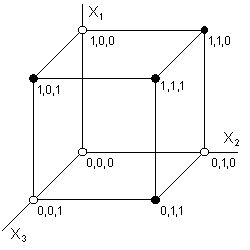
\includegraphics[scale=0.6]{images/Pic_2_1d.png}
\end{center}

Отмечаем точки, на которых функция принимает 1. Заметим, что любой конъюнкт принимает значение 1 на какой-то гиперграни (грани, ребре или вершине для случая $n = 3$). Поэтому пытаемся найти минималное покрытие такими гипергранями. Так и строим.

\subsubsection{Карта Карно}
\href{https://ru.wikipedia.org/wiki/Карта_Карно}{тык}